\subsubsection{Encryption} \label{subsection:counter-replace-encryption-content}
Encryption can be applied on different levels inside the application.
This thesis introduces three different ones.

\subsubsection{Encryption - Resources} \label{subsection:counter-replace-encryption-content-resource}
The first approach is to apply encryption on the application's static resources.
This can include the application's hard coded strings or image assets.
Whenever a resource is used, it has to be decrypted first.
\newline
If application critical strings are encrypted, like server addresses, the application is unable to work without decryption.
If the strings are output strings or pictures, the application will work, but the user will not understand the output, because it is still encrypted and has no meaning to the user.
\newline
Figure~\ref{fig:encryptionResource} shows the abstract implementation of resource decryption.
\begin{figure}[h]
    \centering
    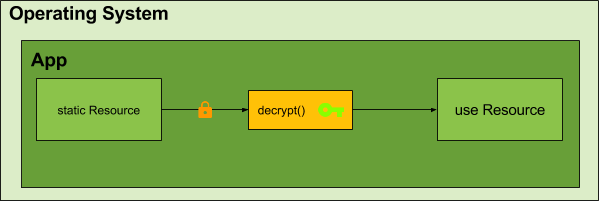
\includegraphics[width=0.8\textwidth]{data/encryptionResource.png}
    \caption{Encrypted resources have to be decrypted before they are used or displayed}
    \label{fig:encryptionResource}
\end{figure}
\newline
There is a possibility to steal decrypted the static resources from authorized applications and insert them unencrypted into a recreated \gls{apk}.
This is a significant effort for a specific application.

\subsubsection{Encryption - Action Obfuscator} \label{subsubsectionection:counter-replace-encryption-content-obfuscator}
The second approach is to use encryption as a form of obfuscation.
The idea is to have a single method (\textit{abstractMethod()}) to delegate all other method calls according to an encrypted parameter.
\newline
When an attacker does a static analysis of the code, the link between the initial call and target method is not apparent.
It forces the attacker to use a dynamic analysis method instead.
The mechanism can be fortified even more, when encrypted arguments are passed.
\newline
An abstract presentation of the mechanism can be seen in figure~\ref{fig:encryptionAction}.
\begin{figure}[h]
    \centering
    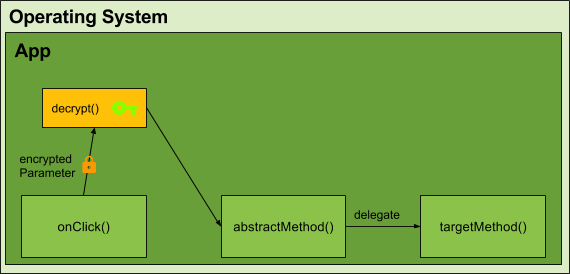
\includegraphics[width=0.8\textwidth]{data/encryptionAction.png}
    \caption{Encrypted paramters to obfuscate method dependencies}
    \label{fig:encryptionAction}
\end{figure}

\subsubsection{Encryption - Communication} \label{section:counter-replace-encryption-content-communication}
The third approach is to use encryption on the server response as seen in figure~\ref{fig:encryptionComm}.
This additional security feature is applied in combination with a content server as described in subsection~\ref{section:counter-replace-server}.
\newline
\begin{figure}[h]
    \centering
    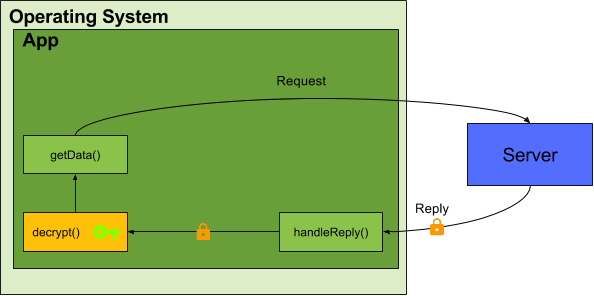
\includegraphics[width=0.8\textwidth]{data/encryptionComm.png}
    \caption{Encrypted communication with a server}
    \label{fig:encryptionComm}
\end{figure}
